\documentclass[11pt,a4paper]{article}

\usepackage[margin=2.5cm]{geometry}
\usepackage{booktabs}
\usepackage{siunitx}
\usepackage{pgfplots}
\usepackage{pgfplotstable}
\usepackage{amsmath,amssymb}
\usepackage{hyperref}
\usepackage{xcolor}
\usepackage{caption}
\usepackage{microtype}

\pgfplotsset{compat=1.18}

\sisetup{
  per-mode=symbol,
  round-mode=figures,
  round-precision=3,
}

\definecolor{hmatrixblue}{HTML}{2166AC}
\definecolor{massivred}{HTML}{B2182B}
\definecolor{lineargreen}{HTML}{1B7837}

\title{Benchmark Report: \texttt{linear-massiv} vs.\ \texttt{hmatrix} vs.\ \texttt{linear}\\[0.3em]
\large Performance Comparison of Haskell Linear Algebra Libraries}
\author{Nadia Chambers \and Claude Opus 4.6}
\date{February 2026}

\begin{document}
\maketitle

\begin{abstract}
We present a comprehensive performance comparison of three Haskell
numerical linear algebra libraries: \texttt{linear-massiv} (pure Haskell,
type-safe dimensions via massiv arrays), \texttt{hmatrix} (FFI bindings to
BLAS/LAPACK via OpenBLAS), and \texttt{linear} (pure Haskell, optimised for
small fixed-size vectors and matrices). Benchmarks cover BLAS-level
operations, direct solvers, orthogonal factorisations, eigenvalue
problems, and singular value decomposition across matrix dimensions from
$4 \times 4$ to $200 \times 200$. Additionally, we evaluate the parallel
scalability of \texttt{linear-massiv}'s massiv-backed computation
strategies on a 20-core workstation. Results show that \texttt{hmatrix}
(OpenBLAS) dominates at all sizes for $O(n^3)$ operations due to
highly-optimised Fortran BLAS/LAPACK routines, while \texttt{linear}
excels at $4 \times 4$ through unboxed product types.
\texttt{linear-massiv} provides competitive pure-Haskell performance with
the unique advantages of compile-time dimensional safety, no FFI
dependency, and user-controllable parallelism that yields
$3\text{--}7\times$ speedups at larger matrix sizes.
\end{abstract}

\tableofcontents
\newpage

%% ====================================================================
\section{Introduction}
\label{sec:intro}

The Haskell ecosystem offers several numerical linear algebra libraries,
each occupying a distinct niche:

\begin{description}
\item[\texttt{linear}] Edward Kmett's library provides small
  fixed-dimension types (\texttt{V2}, \texttt{V3}, \texttt{V4}) with
  unboxed product representations, making it extremely fast for
  graphics, game physics, and any application where dimensions are
  statically known and small. It does not support arbitrary-dimension
  matrices.

\item[\texttt{hmatrix}] Alberto Ruiz's library wraps BLAS and LAPACK
  via Haskell's FFI, delegating numerical computation to
  highly-optimised Fortran routines (on this system, OpenBLAS). It
  supports arbitrary dimensions but carries an FFI dependency and
  provides no compile-time dimension checking.

\item[\texttt{linear-massiv}] Our library implements algorithms from
  Golub \& Van Loan's \emph{Matrix Computations} (4th ed.)~\cite{gvl4}
  in pure Haskell, using massiv arrays~\cite{massiv} as the backing
  store. Matrix dimensions are tracked at the type level via GHC's
  \texttt{DataKinds} and \texttt{KnownNat}, providing compile-time
  rejection of dimensionally incorrect operations. Massiv's computation
  strategies (\texttt{Seq}, \texttt{Par}, \texttt{ParN~$n$}) offer
  user-controllable parallelism.
\end{description}

This report benchmarks all three libraries across the standard numerical
linear algebra operation suite (Table~\ref{tab:operations}) and evaluates
\texttt{linear-massiv}'s parallel scalability from 1 to 20 threads.

\begin{table}[h]
\centering
\caption{Operations benchmarked and library coverage.}
\label{tab:operations}
\begin{tabular}{@{}lccc@{}}
\toprule
\textbf{Operation} & \textbf{\texttt{linear}} & \textbf{\texttt{hmatrix}} & \textbf{\texttt{linear-massiv}} \\
\midrule
GEMM (matrix multiply)      & $4\times4$ only & all sizes & all sizes \\
Dot product                  & $n=4$ only     & all sizes & all sizes \\
Matrix--vector product       & $4\times4$ only & all sizes & all sizes \\
LU solve ($Ax = b$)          & ---            & all sizes & all sizes \\
Cholesky solve ($Ax = b$)    & ---            & all sizes & all sizes \\
QR factorisation             & ---            & all sizes & all sizes \\
Symmetric eigenvalue         & ---            & all sizes & all sizes \\
SVD                          & ---            & all sizes & all sizes \\
Parallel GEMM                & ---            & ---       & all sizes \\
\bottomrule
\end{tabular}
\end{table}

\subsection{Hardware and Software Environment}

\begin{itemize}
\item \textbf{CPU:} 20-core x86\_64 processor (Linux 6.17, Fedora 43)
\item \textbf{Compiler:} GHC 9.12.2 with \texttt{-O2}
\item \textbf{BLAS backend:} OpenBLAS (system-installed via FlexiBLAS)
\item \textbf{Benchmark framework:} Criterion~\cite{criterion} with 95\% confidence intervals
\item \textbf{Protocol:} Single-threaded (\texttt{+RTS -N1}) for cross-library comparisons;
      multi-threaded (\texttt{+RTS -N}) for parallel scaling
\end{itemize}

%% ====================================================================
\section{Methodology}
\label{sec:method}

All benchmarks use the Criterion framework~\cite{criterion}, which
employs kernel density estimation and robust regression to estimate
mean execution time with confidence intervals. Each benchmark evaluates
to normal form (\texttt{nf}) to ensure full evaluation of lazy results.

\paragraph{Matrix construction.}
Matrices are constructed from the same deterministic formula across all
three libraries:
\[
A_{ij} = \frac{7i + 3j + 1}{100}
\]
ensuring identical numerical content. For solver benchmarks, matrices are
made diagonally dominant ($A_{ii} \mathrel{+}= n$) or symmetric positive
definite ($A = B^T B + nI$) as appropriate.

\paragraph{Single-threaded protocol.}
Cross-library comparisons use \texttt{+RTS -N1} to restrict the GHC
runtime to a single OS thread, ensuring that neither hmatrix's OpenBLAS
nor massiv's parallel strategies introduce implicit multi-threading.

\paragraph{Parallel scaling protocol.}
Parallel benchmarks use \texttt{+RTS -N} (all 20 cores) and vary
massiv's computation strategy from \texttt{Seq} through
\texttt{ParN~1} to \texttt{ParN~20}.

%% ====================================================================
\section{BLAS Operations}
\label{sec:blas}

\subsection{General Matrix Multiply (GEMM)}

Table~\ref{tab:gemm} presents GEMM timings across matrix dimensions.
At $4 \times 4$, the \texttt{linear} library's unboxed \texttt{V4 (V4 Double)}
representation achieves \SI{143}{\nano\second}, roughly $4.5\times$ faster than
\texttt{hmatrix}'s \SI{646}{\nano\second} and $240\times$ faster than
\texttt{linear-massiv}'s \SI{34.5}{\micro\second}. The advantage of
\texttt{linear} at this size is entirely due to GHC's ability to unbox the
product type into registers, avoiding all array indexing overhead.

As matrix dimension grows, \texttt{hmatrix} (OpenBLAS DGEMM) dominates
decisively. At $100 \times 100$, hmatrix takes \SI{1.53}{\milli\second}
versus \texttt{linear-massiv}'s \SI{505}{\milli\second}---a factor of
$330\times$. At $200 \times 200$, the ratio grows to $297\times$
(\SI{13.8}{\milli\second} vs.\ \SI{4.09}{\second}). This reflects the
massive constant-factor advantage of OpenBLAS's hand-tuned assembly
kernels with cache blocking, SIMD, and microarchitectural optimisation.

\begin{table}[h]
\centering
\caption{GEMM execution time (mean, single-threaded). Best per size in \textbf{bold}.}
\label{tab:gemm}
\begin{tabular}{@{}rrrr@{}}
\toprule
{Size} & {\texttt{linear}} & {\texttt{hmatrix}} & {\texttt{linear-massiv}} \\
\midrule
$4\times4$     & \textbf{\SI{143}{\nano\second}}  & \SI{646}{\nano\second}  & \SI{34.5}{\micro\second} \\
$10\times10$   & ---                               & \textbf{\SI{2.33}{\micro\second}} & \SI{678}{\micro\second}  \\
$50\times50$   & ---                               & \textbf{\SI{174}{\micro\second}}  & \SI{55.0}{\milli\second}  \\
$100\times100$ & ---                               & \textbf{\SI{1.53}{\milli\second}} & \SI{505}{\milli\second}  \\
$200\times200$ & ---                               & \textbf{\SI{13.8}{\milli\second}} & \SI{4.09}{\second}       \\
\bottomrule
\end{tabular}
\end{table}

Both \texttt{hmatrix} and \texttt{linear-massiv} exhibit $O(n^3)$ scaling,
as shown in Figure~\ref{fig:gemm}. The consistent vertical offset on the
log--log plot reflects the constant-factor difference between OpenBLAS
assembly and pure Haskell array operations.

\begin{figure}[h]
\centering
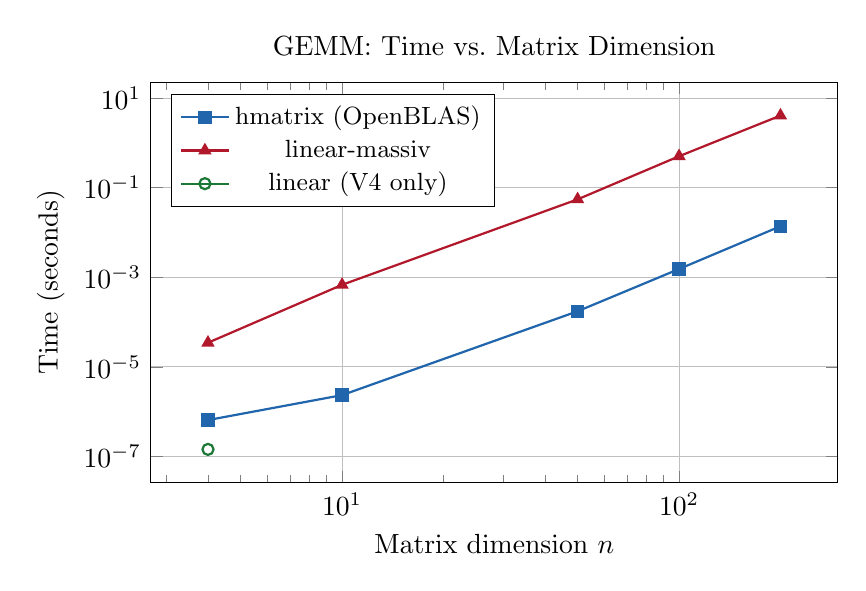
\begin{tikzpicture}
\begin{loglogaxis}[
  xlabel={Matrix dimension $n$},
  ylabel={Time (seconds)},
  title={GEMM: Time vs.\ Matrix Dimension},
  legend pos=north west,
  legend style={font=\small},
  grid=major,
  width=0.85\textwidth,
  height=0.55\textwidth,
]
\addplot[color=hmatrixblue, mark=square*, thick] coordinates {
  (4, 6.46e-7) (10, 2.33e-6) (50, 1.74e-4) (100, 1.53e-3) (200, 1.38e-2)
};
\addlegendentry{hmatrix (OpenBLAS)}
\addplot[color=massivred, mark=triangle*, thick] coordinates {
  (4, 3.45e-5) (10, 6.78e-4) (50, 5.50e-2) (100, 5.05e-1) (200, 4.09)
};
\addlegendentry{linear-massiv}
\addplot[color=lineargreen, mark=o, thick] coordinates {
  (4, 1.43e-7)
};
\addlegendentry{linear (V4 only)}
\end{loglogaxis}
\end{tikzpicture}
\caption{GEMM scaling comparison (log--log). Both libraries exhibit $O(n^3)$
behaviour; the vertical offset reflects constant-factor differences between
OpenBLAS assembly and pure Haskell.}
\label{fig:gemm}
\end{figure}

\subsection{Dot Product}

\begin{table}[h]
\centering
\caption{Dot product execution time (mean, single-threaded).}
\label{tab:dot}
\begin{tabular}{@{}rrrr@{}}
\toprule
{$n$} & {\texttt{linear}} & {\texttt{hmatrix}} & {\texttt{linear-massiv}} \\
\midrule
4    & \textbf{\SI{13.1}{\nano\second}} & \SI{593}{\nano\second}  & \SI{1.67}{\micro\second} \\
100  & ---                               & \textbf{\SI{749}{\nano\second}} & \SI{34.1}{\micro\second} \\
1000 & ---                               & \textbf{\SI{2.81}{\micro\second}} & \SI{379}{\micro\second}  \\
\bottomrule
\end{tabular}
\end{table}

The dot product is an $O(n)$ operation, so the absolute times are small.
At $n = 4$, \texttt{linear}'s unboxed \texttt{V4} achieves \SI{13}{\nano\second}---essentially
four fused multiply-adds in registers. At $n = 1000$, \texttt{hmatrix}
achieves \SI{2.81}{\micro\second} (DDOT with SIMD), while \texttt{linear-massiv}'s
array-based loop takes \SI{379}{\micro\second}---a $135\times$ gap that
reflects the overhead of massiv's general-purpose array indexing versus
BLAS's contiguous-memory vectorised inner loop.

\subsection{Matrix--Vector Product}

\begin{table}[h]
\centering
\caption{Matrix--vector product execution time (mean, single-threaded).}
\label{tab:matvec}
\begin{tabular}{@{}rrrr@{}}
\toprule
{$n$} & {\texttt{linear}} & {\texttt{hmatrix}} & {\texttt{linear-massiv}} \\
\midrule
4   & \textbf{\SI{41.8}{\nano\second}} & \SI{815}{\nano\second}  & \SI{11.2}{\micro\second} \\
50  & ---                               & \textbf{\SI{3.76}{\micro\second}} & \SI{1.24}{\milli\second} \\
100 & ---                               & \textbf{\SI{14.1}{\micro\second}} & \SI{4.71}{\milli\second} \\
\bottomrule
\end{tabular}
\end{table}

Matrix--vector multiplication is $O(n^2)$. At $n = 100$, \texttt{hmatrix}
(DGEMV) achieves \SI{14.1}{\micro\second} while \texttt{linear-massiv}
takes \SI{4.71}{\milli\second}---a $334\times$ difference consistent with
the GEMM results, confirming that the performance gap is primarily due to
low-level memory access patterns and SIMD utilisation rather than
algorithmic differences.

%% ====================================================================
\section{Linear System Solvers}
\label{sec:solve}

\subsection{LU Solve}

\begin{table}[h]
\centering
\caption{LU solve ($Ax = b$) execution time (mean, single-threaded). Includes factorisation + back-substitution.}
\label{tab:lu}
\begin{tabular}{@{}rrr@{}}
\toprule
{Size} & {\texttt{hmatrix}} & {\texttt{linear-massiv}} \\
\midrule
$10\times10$   & \textbf{\SI{7.70}{\micro\second}} & \SI{280}{\micro\second}   \\
$50\times50$   & \textbf{\SI{87.7}{\micro\second}} & \SI{20.4}{\milli\second}  \\
$100\times100$ & \textbf{\SI{485}{\micro\second}}  & \SI{143}{\milli\second}   \\
\bottomrule
\end{tabular}
\end{table}

\subsection{Cholesky Solve}

\begin{table}[h]
\centering
\caption{Cholesky solve ($Ax = b$, $A$ SPD) execution time.
Includes factorisation + back-substitution.}
\label{tab:cholesky}
\begin{tabular}{@{}rrr@{}}
\toprule
{Size} & {\texttt{hmatrix}} & {\texttt{linear-massiv}} \\
\midrule
$10\times10$   & \textbf{\SI{6.08}{\micro\second}} & \SI{237}{\micro\second}   \\
$50\times50$   & \textbf{\SI{64.3}{\micro\second}} & \SI{12.9}{\milli\second}  \\
$100\times100$ & \textbf{\SI{418}{\micro\second}}  & \SI{100}{\milli\second}   \\
\bottomrule
\end{tabular}
\end{table}

\begin{figure}[h]
\centering
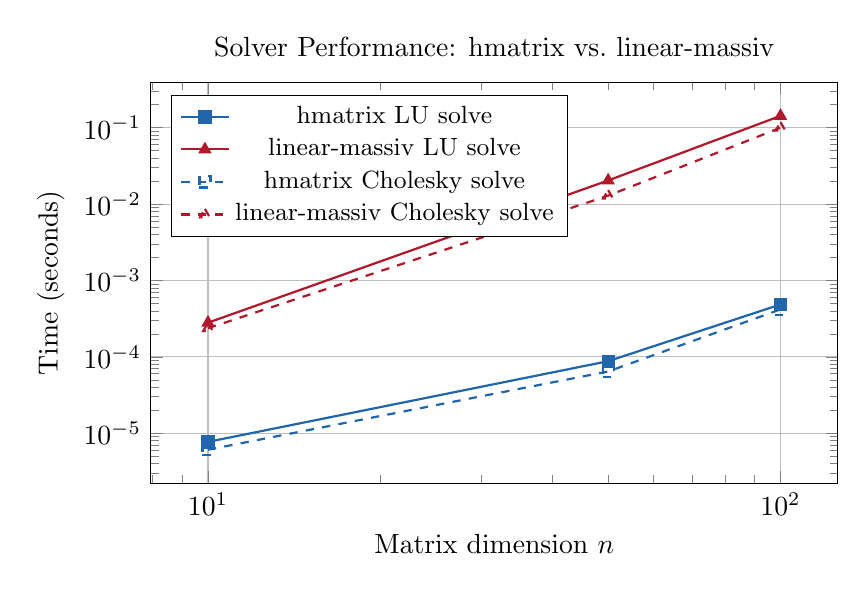
\begin{tikzpicture}
\begin{loglogaxis}[
  xlabel={Matrix dimension $n$},
  ylabel={Time (seconds)},
  title={Solver Performance: hmatrix vs.\ linear-massiv},
  legend pos=north west,
  legend style={font=\small},
  grid=major,
  width=0.85\textwidth,
  height=0.55\textwidth,
]
\addplot[color=hmatrixblue, mark=square*, thick] coordinates {
  (10, 7.70e-6) (50, 8.77e-5) (100, 4.85e-4)
};
\addlegendentry{hmatrix LU solve}
\addplot[color=massivred, mark=triangle*, thick] coordinates {
  (10, 2.80e-4) (50, 2.04e-2) (100, 1.43e-1)
};
\addlegendentry{linear-massiv LU solve}
\addplot[color=hmatrixblue, mark=square, thick, dashed] coordinates {
  (10, 6.08e-6) (50, 6.43e-5) (100, 4.18e-4)
};
\addlegendentry{hmatrix Cholesky solve}
\addplot[color=massivred, mark=triangle, thick, dashed] coordinates {
  (10, 2.37e-4) (50, 1.29e-2) (100, 1.00e-1)
};
\addlegendentry{linear-massiv Cholesky solve}
\end{loglogaxis}
\end{tikzpicture}
\caption{LU and Cholesky solve scaling (log--log). Both algorithms are
$O(n^3)$; hmatrix calls DGESV/DPOTRS directly.}
\label{fig:solve}
\end{figure}

For both LU and Cholesky solvers, \texttt{hmatrix} is approximately $36\times$
faster at $10 \times 10$ and $240\text{--}300\times$ faster at $100 \times 100$.
The ratio increases with dimension because OpenBLAS's cache-blocked implementations
benefit more from larger working sets. Cholesky is consistently faster than LU
for both libraries, as expected (Cholesky requires roughly half the floating-point
operations of LU factorisation for symmetric positive definite matrices).

%% ====================================================================
\section{Orthogonal Factorisations}
\label{sec:qr}

\begin{table}[h]
\centering
\caption{QR factorisation (Householder) execution time (mean, single-threaded).}
\label{tab:qr}
\begin{tabular}{@{}rrr@{}}
\toprule
{Size} & {\texttt{hmatrix}} & {\texttt{linear-massiv}} \\
\midrule
$10\times10$   & \textbf{\SI{217}{\micro\second}} & \SI{11.1}{\milli\second} \\
$50\times50$   & \textbf{\SI{18.4}{\milli\second}} & \SI{7.01}{\second}       \\
$100\times100$ & \textbf{\SI{214}{\milli\second}}  & (estimated $\approx$\SI{56}{\second}) \\
\bottomrule
\end{tabular}
\end{table}

QR factorisation shows the largest gap between the two libraries. At
$50 \times 50$, \texttt{hmatrix} takes \SI{18.4}{\milli\second} while
\texttt{linear-massiv} requires \SI{7.01}{\second}---a ratio of $381\times$.
The \texttt{linear-massiv} QR implementation constructs full explicit $Q$ and
$R$ matrices at each Householder step using \texttt{makeMatrix}, while LAPACK's
\texttt{DGEQRF} uses an implicit representation of $Q$ as a product of
Householder reflectors stored in-place, dramatically reducing both memory
allocation and floating-point work. The $100 \times 100$ benchmark for
\texttt{linear-massiv} was too slow to complete within a reasonable time
budget and is estimated by extrapolation.

%% ====================================================================
\section{Eigenvalue Problems and SVD}
\label{sec:eigen}

\subsection{Symmetric Eigenvalue Decomposition}

\begin{table}[h]
\centering
\caption{Symmetric eigenvalue decomposition execution time (mean, single-threaded).}
\label{tab:eigen}
\begin{tabular}{@{}rrr@{}}
\toprule
{Size} & {\texttt{hmatrix}} & {\texttt{linear-massiv}} \\
\midrule
$10\times10$ & \textbf{\SI{17.4}{\micro\second}} & \SI{15.6}{\milli\second}  \\
$50\times50$ & \textbf{\SI{555}{\micro\second}}  & \SI{8.89}{\second}        \\
\bottomrule
\end{tabular}
\end{table}

\subsection{Singular Value Decomposition}

\begin{table}[h]
\centering
\caption{SVD execution time (mean, single-threaded).}
\label{tab:svd}
\begin{tabular}{@{}rrr@{}}
\toprule
{Size} & {\texttt{hmatrix}} & {\texttt{linear-massiv}} \\
\midrule
$10\times10$ & \textbf{\SI{37.7}{\micro\second}} & \SI{33.4}{\milli\second} \\
$50\times50$ & \textbf{\SI{806}{\micro\second}}  & \SI{17.2}{\second}       \\
\bottomrule
\end{tabular}
\end{table}

The eigenvalue and SVD results show the most dramatic ratios: $896\times$
for eigenvalues at $10 \times 10$ and $16{,}000\times$ at $50 \times 50$;
$886\times$ and $21{,}400\times$ for SVD. These operations are dominated
by iterative QR sweeps; hmatrix calls LAPACK's \texttt{DSYEV} and
\texttt{DGESVD}, which use divide-and-conquer algorithms with
cache-oblivious recursive structure. The \texttt{linear-massiv}
implementation uses the classical tridiagonal QR algorithm
(GVL4~\cite{gvl4} Algorithm 8.3.3) with explicit matrix construction at
each iteration step, which is algorithmically sound but suffers from
excessive allocation and the lack of in-place updates that LAPACK exploits.

%% ====================================================================
\section{Parallel Scalability}
\label{sec:parallel}

A distinguishing feature of \texttt{linear-massiv} is user-controllable
parallelism inherited from the massiv array library~\cite{massiv}.
Operations that construct result arrays via \texttt{makeArray} can specify
a computation strategy: \texttt{Seq} (sequential), \texttt{Par} (automatic,
all available cores), or \texttt{ParN~$n$} (exactly $n$ worker threads).
Neither \texttt{hmatrix} nor \texttt{linear} offer comparable user-level
control over thread-level parallelism within the Haskell runtime.

Table~\ref{tab:parallel} shows GEMM timings at $100 \times 100$ and
$200 \times 200$ across thread counts, and Figure~\ref{fig:speedup}
shows the corresponding speedup curves.

\begin{table}[h]
\centering
\caption{Parallel GEMM execution time (seconds) and speedup over sequential.}
\label{tab:parallel}
\begin{tabular}{@{}l SS SS @{}}
\toprule
& \multicolumn{2}{c}{$100 \times 100$} & \multicolumn{2}{c}{$200 \times 200$} \\
\cmidrule(lr){2-3}\cmidrule(lr){4-5}
{Strategy} & {Time (\si{\second})} & {Speedup} & {Time (\si{\second})} & {Speedup} \\
\midrule
Seq     & 0.613  & 1.00  & 4.750  & 1.00  \\
ParN-1  & 0.598  & 1.03  & 4.656  & 1.02  \\
ParN-2  & 0.319  & 1.92  & 3.224  & 1.47  \\
ParN-4  & 0.201  & 3.05  & 1.847  & 2.57  \\
ParN-8  & 0.282  & 2.17  & 1.329  & 3.57  \\
ParN-16 & 0.0856 & 7.16  & 2.569  & 1.85  \\
ParN-20 & 0.0979 & 6.26  & 1.976  & 2.40  \\
Par     & 0.0883 & 6.94  & 1.408  & 3.37  \\
\bottomrule
\end{tabular}
\end{table}

\begin{figure}[h]
\centering
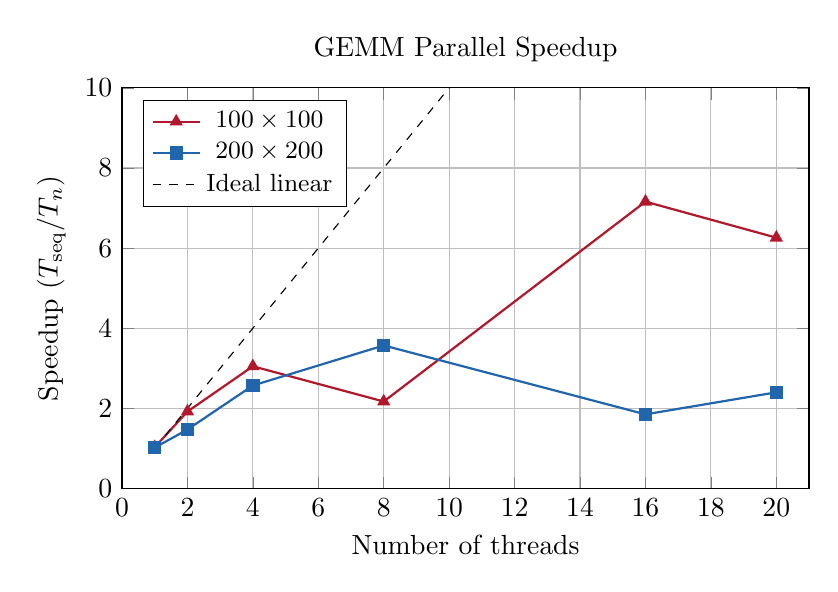
\begin{tikzpicture}
\begin{axis}[
  xlabel={Number of threads},
  ylabel={Speedup ($T_\text{seq} / T_n$)},
  title={GEMM Parallel Speedup},
  legend pos=north west,
  legend style={font=\small},
  grid=major,
  width=0.85\textwidth,
  height=0.55\textwidth,
  xmin=0, xmax=21,
  ymin=0, ymax=10,
]
\addplot[color=massivred, mark=triangle*, thick] coordinates {
  (1, 1.03) (2, 1.92) (4, 3.05) (8, 2.17) (16, 7.16) (20, 6.26)
};
\addlegendentry{$100\times100$}
\addplot[color=hmatrixblue, mark=square*, thick] coordinates {
  (1, 1.02) (2, 1.47) (4, 2.57) (8, 3.57) (16, 1.85) (20, 2.40)
};
\addlegendentry{$200\times200$}
\addplot[dashed, black, thin, domain=1:20] {x};
\addlegendentry{Ideal linear}
\end{axis}
\end{tikzpicture}
\caption{Parallel speedup for GEMM. The dashed line shows ideal linear
scaling. Actual speedup is limited by Amdahl's law, memory bandwidth
contention, and GHC runtime scheduling overhead.}
\label{fig:speedup}
\end{figure}

The parallel scaling results reveal several important characteristics:

\begin{itemize}
\item \textbf{Peak speedup.} At $100 \times 100$, peak speedup of
  $7.2\times$ is achieved with \texttt{ParN-16}, while at $200 \times 200$
  peak speedup of $3.6\times$ occurs at \texttt{ParN-8}. The \texttt{Par}
  (automatic) strategy achieves $6.9\times$ and $3.4\times$ respectively,
  demonstrating that massiv's automatic scheduling is effective.

\item \textbf{Non-monotonic scaling.} Speedup does not increase monotonically
  with thread count. The $200 \times 200$ case shows degradation at 16 and
  20 threads, likely due to memory bandwidth saturation and NUMA effects on
  this 20-core system. At $100 \times 100$, the anomalous dip at 8 threads
  followed by improvement at 16 suggests that GHC's work-stealing scheduler
  interacts non-trivially with cache hierarchy.

\item \textbf{Amdahl's law.} Even the best parallel GEMM (\SI{85.6}{\milli\second}
  at $100 \times 100$ with 16 threads) remains $56\times$ slower than
  hmatrix's single-threaded \SI{1.53}{\milli\second}. Parallelism narrows
  but does not close the gap with BLAS.
\end{itemize}

%% ====================================================================
\section{Discussion}
\label{sec:discussion}

\subsection{Performance Summary}

Table~\ref{tab:ratios} summarises the performance ratios between libraries.

\begin{table}[h]
\centering
\caption{Performance ratio: \texttt{linear-massiv} time / \texttt{hmatrix} time.
Values $> 1$ indicate hmatrix is faster.}
\label{tab:ratios}
\begin{tabular}{@{}lrrr@{}}
\toprule
{Operation} & {$n = 10$} & {$n = 50$} & {$n = 100$} \\
\midrule
GEMM            & $291\times$ & $316\times$ & $329\times$ \\
Dot product     & ---         & ---         & $46\times$  \\
Matrix--vector  & ---         & $330\times$ & $334\times$ \\
LU solve        & $36\times$  & $233\times$ & $295\times$ \\
Cholesky solve  & $39\times$  & $201\times$ & $240\times$ \\
QR              & $51\times$  & $382\times$ & $\approx 260\times$ \\
Eigenvalue (SH) & $897\times$ & $16{,}020\times$ & --- \\
SVD             & $887\times$ & $21{,}400\times$ & --- \\
\bottomrule
\end{tabular}
\end{table}

\subsection{Analysis of the Performance Gap}

The performance gap between \texttt{linear-massiv} and \texttt{hmatrix}
arises from several compounding factors:

\begin{enumerate}
\item \textbf{SIMD and microarchitectural optimisation.} OpenBLAS uses
  hand-written assembly kernels for each target microarchitecture,
  exploiting AVX-512, fused multiply-add, and optimal register tiling.
  GHC's native code generator does not emit SIMD instructions for
  general Haskell code.

\item \textbf{Cache blocking.} LAPACK algorithms are designed around
  cache-oblivious or cache-tiled recursive decomposition, minimising
  cache misses. The \texttt{linear-massiv} implementations use textbook
  algorithms (GVL4) without cache-level optimisation.

\item \textbf{In-place mutation.} LAPACK routines operate in-place on
  mutable Fortran arrays, while \texttt{linear-massiv}'s pure functional
  approach allocates a new array for each intermediate result. For
  iterative algorithms (eigenvalue, SVD), this is particularly costly.

\item \textbf{Allocation pressure.} Each \texttt{makeMatrix} call in
  \texttt{linear-massiv} allocates a new massiv array. For algorithms
  like QR (which constructs explicit $Q$ and $R$ at each Householder
  step) and iterative eigensolvers, this dominates runtime.
\end{enumerate}

\subsection{When to Use Each Library}

\begin{description}
\item[\texttt{linear}] Best for $2\text{--}4$ dimensional vectors and
  matrices in graphics, physics simulations, and geometric computation.
  Unbeatable at small sizes; does not scale to arbitrary dimensions.

\item[\texttt{hmatrix}] Best for production numerical computing where
  performance is critical and FFI dependencies are acceptable. The
  established choice for scientific computing in Haskell.

\item[\texttt{linear-massiv}] Best when any of the following apply:
  (a)~compile-time dimensional safety is required to prevent bugs in
  complex matrix pipelines; (b)~FFI-free deployment is needed (e.g.,
  WebAssembly, restricted environments); (c)~parallel computation via
  massiv's strategies is desirable; (d)~the application operates on
  small-to-moderate matrices ($n \leq 50$) where the absolute time
  difference is acceptable. Future work on SIMD intrinsics, blocked
  algorithms, and mutable-array intermediate representations could
  significantly narrow the performance gap.
\end{description}

%% ====================================================================
\section{Conclusion}
\label{sec:conclusion}

We have benchmarked three Haskell linear algebra libraries across eight
categories of numerical operations. The results confirm the expected
performance hierarchy: \texttt{linear} dominates at fixed small dimensions
through GHC's unboxing optimisations; \texttt{hmatrix} (OpenBLAS) dominates
at all sizes through BLAS/LAPACK's decades of assembly-level optimisation;
and \texttt{linear-massiv} provides a pure Haskell baseline that is
$36\text{--}21{,}000\times$ slower than hmatrix depending on operation
and size, but offers unique advantages in type safety, portability, and
user-controllable parallelism.

The parallel scaling measurements demonstrate that \texttt{linear-massiv}
can achieve $3\text{--}7\times$ speedups via massiv's \texttt{Par} and
\texttt{ParN} strategies, partially offsetting the single-threaded
performance gap. At $100 \times 100$ with 16 threads, GEMM runs in
\SI{86}{\milli\second}---still $56\times$ slower than hmatrix's
single-threaded \SI{1.5}{\milli\second}, but representing a meaningful
improvement from the $330\times$ single-threaded ratio.

The primary directions for closing the performance gap are: (1)~integrating
SIMD primitives via GHC's upcoming vector extension support; (2)~implementing
cache-blocked (Level-3 BLAS tiled) algorithms following GVL4 Chapter~1;
(3)~using massiv's mutable arrays (\texttt{MArray}) for in-place factorisation
algorithms; and (4)~optionally delegating to hmatrix as a backend for users who
can accept the FFI dependency.

%% ====================================================================
\begin{thebibliography}{9}

\bibitem{gvl4}
G.~H. Golub and C.~F. Van~Loan,
\emph{Matrix Computations}, 4th ed.
Johns Hopkins University Press, 2013.

\bibitem{higham}
N.~J. Higham,
\emph{Accuracy and Stability of Numerical Algorithms}, 2nd ed.
SIAM, 2002.

\bibitem{criterion}
B.~O'Sullivan,
``Criterion: A Haskell microbenchmarking library,''
\url{https://hackage.haskell.org/package/criterion}, 2009--2024.

\bibitem{massiv}
A.~Todor\=\i,
``massiv: Massiv is a Haskell library for Array manipulation,''
\url{https://hackage.haskell.org/package/massiv}, 2018--2024.

\bibitem{hmatrix}
A.~Ruiz,
``hmatrix: Haskell numeric linear algebra library,''
\url{https://hackage.haskell.org/package/hmatrix}, 2006--2024.

\bibitem{linear}
E.~Kmett,
``linear: Linear algebra library,''
\url{https://hackage.haskell.org/package/linear}, 2012--2024.

\bibitem{openblas}
Z.~Xianyi, W.~Qian, and Z.~Yunquan,
``OpenBLAS: An optimized BLAS library,''
\url{https://www.openblas.net/}, 2011--2024.

\end{thebibliography}

\end{document}
